% !TEX root = thesis.tex

\section{HCCT Construction and Accuracy}
\label{ss:hcct-eval}

In this section, we present an extensive experimental study of our data streaming-based methodology for context-sensitive profiling. We implemented several variants of context-sensitive profilers and we analyzed their performance and the accuracy of the produced $(\phi,\varepsilon)$-HCCT with respect to a number of metrics and using many different parameter settings. Besides the exhaustive approach, where each routine call and return is instrumented, we integrate our solution with previous techniques aimed at reducing time overhead: we focus in particular on static bursting~\cite{Zhuang06}, which offers convenient time-accuracy trade-offs. The experimental analysis not only confirms, but reinforces the theoretical prediction: the $(\phi,\varepsilon)$-HCCT represents the hot portions of the full CCT very well using only an extremely small percentage of the space required by the entire CCT: all the hottest calling contexts are always identified correctly, their counters are very accurate, and the number of false positives is rather small. With bursting, the running time overhead can be kept under control without affecting accuracy in a substantial way.

\subsection{Implementation}
\label{ss:hcct-implementation}

\paragraph*{Compiler Plugin.} The \gcc\ compiler provides an instrumentation infrastructure to emit calls to analysis routines at the beginning and at the end of each function, passing as arguments the address of the current function and its calling site. On top of these two primitives, we have built a full-fledged infrastructure for context sensitive profiling of multi-threaded Linux C/C++ applications that ships as a plugin\footnote{Source code and documentation are available at: \url{https://github.com/dcdelia/hcct}} for the GNU Compiler Collection.

Our plugin provides native support for techniques aimed at reducing run-time overhead, such as sampling and bursting, and does not require modifications to the existing {\tt gcc} installation or to the program to be analyzed (except for its {\tt Makefile}). When a program is compiled, instrumentation is injected into the code by the compiler and the executable is eventually linked against a generic profiling library named {\tt libhcct}. When a user wants to analyze the behavior of an instrumented program, it is possible to switch between different techniques -- including the canonical CCT construction -- or parameter settings with no need to further recompile the code.

\paragraph*{Data Structures.} We use a first-child, next-sibling representation for calling context tree nodes. Each MCCT node also contains a pointer to its parent, the routine ID, the call site, and the performance metric. The first-child, next-sibling representation is space-efficient and still guarantees that the children of each node can be explored in time proportional to their number. According to our experiments with several benchmarks, the average number of scanned children is a small constant around 2-3, so this representation turns out to be convenient also for checking whether a routine ID already appears among the children of a node. The parent field, which is needed to perform tree pruning efficiently (see \myalgorithm\ref{alg:hcct-update} in \mysection\ref{ss:hcct-algorithms}), is not required in CCT nodes. As a routine ID, we simply use the routine address. Overall, CCT and MCCT nodes require 20 and 24 bytes, respectively, on 32 bit architectures. Using a simple bit packing technique~\cite{Standish80}, we also encode in one of the pointer fields a Boolean flag that tells whether the calling context associated with the node is monitored in the streaming data structure M, without increasing the number of bytes per node. To improve time and space efficiency, we allocate nodes through a custom, page-based allocator, which maintains blocks of fixed size. Any additional algorithm-specific information needed to maintain the heavy hitters is stored as trailing fields within MCCT nodes.

\paragraph*{Integration with Static Bursting.} Static bursting~\cite{Zhuang06} is a profiling technique that combines the advantages of sampling-based and exhausting profiling mechanisms. As in sampling-based solutions, a bursting profiler lets a program run unhindered between sampling points, and performs stack walking to determine the current calling context when a sampling point is reached. Rather than incrementing the counter for the corresponding node (which may not reflect an actual function call and thus lead to misleading results), a bursting profiler performs exhaustive instrumentation on the sequence (i.e.,  burst) of call/return events collected in an interval whose length we refer to as {\em burst length}. Further refinement of static bursting are possible, e.g., analysis overhead can be further reduced by selectively disabling bursts for previously sampled calling-contexts and then probabilistically re-enabling them~\cite{Zhuang06}. In our setting, driven by the shadow stack maintained by the profiling infrastructure, we update our cursor pointer by walking down the tree from its root. Missing nodes are initialized and added to the tree during the walk. The execution stream we observe is thus partitioned into bursts and sequences that are transparent to profiling.

\paragraph*{Other Software.} As part of our infrastructure, we have developed two additional pieces of software that might be of independent interest: a library for resolving addresses to symbols, and a set of tools for the analysis and comparison of CCTs from distinct executions. In general, even for deterministic benchmarks it might not be trivial to line up nodes from two executions, as due to technical respects such as address space randomization and dynamic loading of libraries, program addresses can change. In some cases it is not always possible to resolve addresses offline up to a source-file line-number granularity, but the available information is only partial (e.g., we know only the source file where the method is defined). If this happens for two or more sibling nodes that have identical frequency counters, lining them up with tree nodes from another execution requires a similarity analysis of their spanned subtrees. We observed similar scenarios frequently in our experiments, both for hot and cold calling contexts. Since spanned subtrees for CCT nodes can be large, rapid and accurate heuristics are required to summarize the subtrees and compute their similarity; accuracy of heuristics is even more crucial when comparing a CCT with a HCCT, as spanned subtrees in the latter might have been partially or entirely pruned. Using combinatorial techniques and ad-hoc heuristics based on topological properties of the trees, we were able to quickly (i.e., in a few minutes) reconstruct for all our experiments a full and accurate mapping between pairs of different trees.

\subsection{Experimental Setup}
\label{ss:hcct-experimental-setup}

In this section we present the details of our experimental methodology, focusing on benchmarks and accuracy metrics, and we describe how the parameters of the streaming algorithms can be tuned.

\subsubsection*{Benchmarks}
%We performed our tests on a variety of large-scale Linux applications and on a set benchmarks drawn from the \phoronixpts~\cite{Henning06} and the \speccpu~\cite{Henning06} test suites. 
%To ensure deterministic replay of the execution of the interactive applications, we used the PIN dynamic instrumentation framework~\cite{Luk05} to record timestamped execution traces for typical usage sessions of approximately fifteen minutes.
We performed our tests on a variety of large-scale Linux applications, and on benchmarks from the \phoronixpts~\cite{Henning06} and \speccpu~\cite{Henning06} suites with CCTs of at least $100\,000$ nodes. To support execution replay for interactive applications, we used the PIN dynamic instrumentation framework~\cite{Luk05} to record timestamped execution traces for typical usage sessions of approximately fifteen minutes.

Interactive applications include graphics programs ({\tt inkscape} and {\tt gimp}), a hexadecimal file viewer ({\tt ghex2}), audio players/editors ({\tt amarok} and {\tt audacity}), an archiver ({\tt ark}), an Internet browser ({\tt firefox}), an HTML editor ({\tt quanta}), a chat program ({\tt pidgin}), the OpenOffice suite for word processing ({\tt oowriter}), spreadsheets ({\tt oocalc}), and drawing ({\tt ooimpress}).

Non-interactive benchmarks include a cryptographic library ({\tt botan}), a 2D graphics library ({\tt cairo-perf-trace}), advanced chess engines ({\tt crafty} and {\tt sjeng}), the Connect Four ({\tt fhourstones}) and Go ({\tt gobmk}) games, and two 3D games run in demo mode (PlanetPenguin Racer in the {\tt ice-labyrinth} and {\tt mount-herring} scenarios, and SuperTuxKart on the {\tt overworld} and {\tt scotland} tracks).

Statistical information about test sets are reported in \mytable\ref{tab:hcct-CCTsize}\ifauthorea{}{ (page~\pageref{tab:hcct-CCTsize})}: even short sessions result in CCTs consisting of tens of millions of calling contexts, whereas the call graph has only a few thousand nodes. We also observe that the number of distinct call sites is roughly one order of magnitude larger than the call graph.

\subsubsection*{Metrics}
Besides memory usage and time consumption of our profiler, we test the accuracy of the $(\phi,\varepsilon)$-HCCT according to a variety of metrics.

\begin{enumerate}
\item Degree of overlap~\cite{Arnold01,Arnold00,Zhuang06} measures the completeness of the $(\phi,\varepsilon)$-HCCT with respect to the full CCT:
\begin{small}
$$overlap((\phi,\varepsilon){\mbox{-HCCT,\,CCT}})=\frac{1}{N}\sum_{\mbox{\footnotesize{arcs}}~e\in (\phi,\varepsilon)\mbox{\tiny -HCCT}}w(e)$$\\
\end{small}
where $N$ is the total number of routine activations (corresponding to the CCT total weight) and $w(e)$ is the true frequency of the target node of arc $e$ in the CCT.

\item Hot edge coverage~\cite{Zhuang06} measures the percentage of CCT hot edges covered by the $(\phi,\varepsilon)$-HCCT, using an edge-weight threshold $\tau\in [0,1]$ to determine hotness. Since $(\phi,\varepsilon)$-HCCT$\subseteq$CCT, hot edge coverage can be defined as follows:
\begin{small}
$$\hspace{-0mm}cover((\phi,\varepsilon){\mbox{-HCCT,\,CCT}},\tau)=\frac{|\{e\in(\phi,\varepsilon){\mbox{-HCCT:}}\,w(e)\ge\tau \cdot w_{max}\}|}{|\{e\in\mbox{CCT:}\,w(e)\ge\tau \cdot w_{max}\}|}$$\\
\end{small}
where $w_{max}$ is the weight of the hottest CCT arc.

\item Maximum hotness of uncovered calling contexts, where a context is uncovered if is not included in the $(\phi,\varepsilon)$-HCCT:
\begin{small}
$$maxUncov((\phi,\varepsilon){\mbox{-HCCT,\,CCT}})=\max_{e\in\mbox{\tiny CCT}\setminus(\phi,\varepsilon){\mbox{\tiny -HCCT}}}\frac{w(e)}{w_{max}}\times 100$$\\
\end{small}
Average hotness of uncovered contexts is defined similarly.

\item Number of false positives, i.e., $|A\setminus H|$: the smaller this number, the better the $(\phi,\varepsilon){\mbox{-HCCT}}$ approximates the exact HCCT obtained from CCT pruning.

\item Maximum counter error, i.e., maximum error in the frequency counters of $(\phi,\varepsilon)$-HCCT nodes with respect to their true value in the full CCT:
\begin{small}
$$maxError((\phi,\varepsilon){\mbox{-HCCT}})=\max_{e\in(\phi,\varepsilon){\mbox{\tiny -HCCT}}}\frac{|w(e)-\widetilde{w}(e)|}{w(e)}\times 100$$\\
\end{small}
where $w(e)$ and $\widetilde{w}(e)$ are the true and the estimated frequency of context $e$, respectively. Average counter error is defined similarly.
\end{enumerate}

\noindent We remark that an accurate solution should maximize (1) and (2), and minimize the remaining metrics.

\subsubsection*{Parameter Tuning}

Before describing our experimental findings, we discuss how to choose parameters $\phi$ and $\varepsilon$ to be provided as input to the streaming algorithms. According to the theoretical analysis, an accurate choice of $\phi$ and $\varepsilon$  might greatly affect the space used by the algorithms and the accuracy of the solution. In our study we considered many different choices of $\phi$ and $\varepsilon$ across rather heterogeneous sets of benchmarks and execution traces, always obtaining similar results that we summarize below. 

A rule of thumb about $\phi$ and $\varepsilon$ validated by previous experimental studies~\cite{Cormode08} suggests that it is sufficient to choose $\varepsilon=\phi/10$ in order to obtain high counter accuracy and a small number of false positives.

We found this choice overly pessimistic in our scenario: the extremely skewed cumulative distribution of calling context frequencies shown in \myfigure\ref{fig:hcct-skewness} \ifauthorea{}{(page \pageref{fig:hcct-skewness})} makes it possible to use much larger values of $\varepsilon$ without sacrificing accuracy. This yields substantial benefits on the space usage, which is roughly proportional to $1/\varepsilon$. Unless otherwise stated, in all our experiments we used $\varepsilon=\phi/5$.

Let us now consider the choice of $\phi$: $\phi$ is the hotness threshold with respect to the stream length $N$, i.e., to the number of routine enter events. However, $N$ is unknown {\em a priori} during profiling, and thus choosing $\phi$ appropriately may appear to be difficult: too-large values might result in returning very few hot calling contexts (even no context at all in some extreme cases), while too-small values might result in using too much space and returning too many contexts without being able to discriminate accurately which of them are actually hot. Our experiments suggest that an appropriate choice of $\phi$ is mostly independent of the specific benchmark and of the stream length: as shown in \mytable\ref{tab:hcct-phi}, different benchmarks have HCCT sizes of the same order of magnitude when using the same $\phi$ threshold (results for omitted benchmarks are similar). This is a consequence of the skewness of context frequency distribution, and greatly simplifies the choice of $\phi$ in practice. Unless otherwise stated, in our experiments we used $\phi=10^{-4}$, which corresponds to mining roughly the hottest 1,000 calling contexts independently of the benchmark.

\begin{table}[ht]
\vspace{2mm}
\begin{center}
\begin{tabular}{c c c c c}
\hline
  & HCCT nodes  & HCCT nodes & HCCT nodes & CCT nodes \\ 
Benchmark & $\phi=10^{-3}$  & $\phi=10^{-5}$ & $\phi=10^{-7}$ \\ 
\hline
audacity & 112 & 9\,181 & 233\,362 & 13\,131\,115 \\
dolphin & 97 & 14\,563 & 978\,544 & 11\,667\,974 \\
gimp & 96 & 15\,330 & 963\,708 & 26\,107\,261 \\
ice-labyrinth & 93 & 9\,413 & 529\,945 & 2\,160\,052 \\
inkscape & 80 & 16\,713 & 830\,191 & 13\,896\,175 \\
oocalc & 136 & 13\,414 & 1\,339\,752 & 48\,310\,585 \\
quanta & 94 & 13\,881 & 812\,098 & 27\,426\,654 \\
\hline
\end{tabular}
\vspace{3mm}
\caption{\label{tab:hcct-phi} Typical thresholds for calling context frequencies.}
\end{center}
\end{table}
\ifauthorea{\newline}{}

\subsubsection*{Platform}

In our experiments we used a 2.53GHz Intel Core2 Duo T9400 with 128KB of L1 data cache, 6MB of L2 cache, and 4 GB of main memory DDR3 1066, running Ubuntu 12.04, Linux Kernel 3.5.0, gcc 4.7.2, 32 bit. We collected performance measurements with negligible background activity, running multiple trials for each benchmark/tool combination and reporting confidence intervals stated at 95\% confidence level.

\subsection{Memory Usage}
\label{ss:eval-hcct-memory}

We first evaluate how much space can be saved by our approach, reporting the size of the MCCT constructed by the SS algorithm compared to the size of the full CCT as a function of the hotness threshold $\phi$. \myfigure\ref{fig:hcct-space-by-phi} shows the results for a representative subset of benchmarks. Notice that the size of the MCCT, hence the space used by the algorithm, decreases with $\phi$. For values of $\phi\ge 10^{-4}$, i.e., contexts that appear at least $0.01\%$ of the time, space usage remains less than $1\%$ than the CCT size for most benchmarks, with a worst case of about $4.1\%$ over all our experiments.

\ifdefined\noauthorea
\begin{figure}[!ht]
\begin{center}
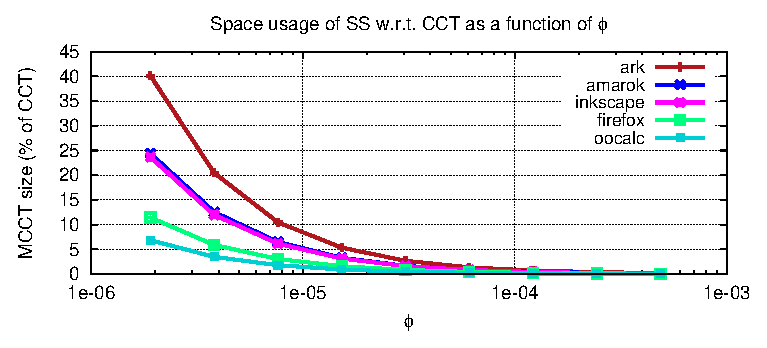
\includegraphics[width=0.75\textwidth]{figures/hcct-space-by-phi/hcct-space-by-phi.eps}
\caption{\protect\label{fig:hcct-space-by-phi} Space usage as a function of the hotness threshold $\phi$..
}
\end{center}
\end{figure}
\fi

\ifdefined\noauthorea
\begin{figure}[!ht]
\begin{center}
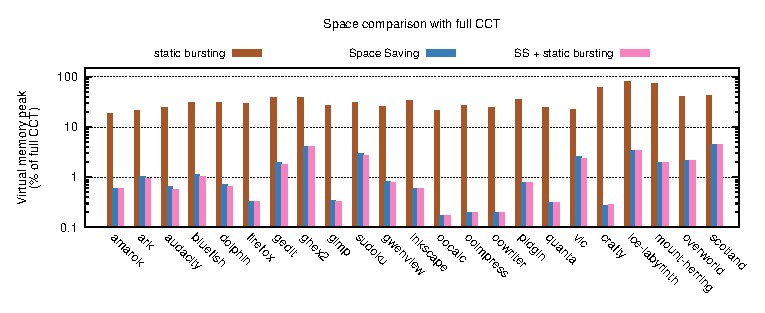
\includegraphics[width=\textwidth]{figures/hcct-space/hcct-space.eps}
\caption{\protect\label{fig:hcct-space} Space analysis of static bursting (left), SS (center), and SS combined with static bursting (right) with sampling interval 2 msec and burst length 0.2 msec.

%Space analysis on several benchmarks of static bursting~\cite{Zhuang06} (left), SS (center), and SS combined with static bursting (right) with sampling interval 2 msec and burst length 0.2 msec.

}
\end{center}
\end{figure}
\fi

As a second experiment, we study the actual memory footprint of our profilers considering both SS and the combination of SS with static bursting. \myfigure\ref{fig:hcct-space} plots the peak memory usage of our profilers as a percentage of the full CCT. We recall that during the computation we store the minimal subtree MCCT of the CCT spanning all monitored contexts. This subtree is eventually pruned to obtain the $(\phi,\varepsilon)$-HCCT (\mysection\ref{ss:hcct-approach,ss:hcct-algorithms}). The peak memory usage is proportional to the number of MCCT nodes, which is typically much larger than the actual number of hot contexts obtained after pruning.

Quite surprisingly, static bursting also improves space usage. This depends on the fact that sampling reduces the variance of calling context frequencies: MCCT cold nodes that have a hot descendant are more likely to become hot when sampling is active, and monitoring these nodes reduces the total MCCT size. The histogram also shows that static bursting alone (i.e., without streaming) is not sufficient to substantially reduce space: in addition to hot contexts, a large fraction of cold contexts is also sampled and included in the CCT. We also observed that the larger the applications, the larger the space reduction of our approach over bursting alone.

Since the average node degree is a small constant, cold HCCT nodes are typically a fraction of the total number of nodes, as shown in \myfigure\ref{fig:hcct-breakdown} for $\phi=10^{-4}$\ifauthorea{}{ (page \pageref{fig:hcct-breakdown})}. In our experiments we observed that this fraction strongly depends on the  hotness threshold $\phi$, and in particular decreases with $\phi$: cold nodes that have a hot descendant are indeed more likely to become hot when $\phi$ is smaller.

\subsection{Time Overhead}

We now discuss the time overhead of our approach, both alone and in combination with static bursting. We compare to native execution, to the widely used call-graph profiler \gprof~\cite{Graham82}, and to the canonical CCT construction. To assess the instrumentation overhead, we also compare to {\em empty} instrumentation (i.e., when no analysis is performed).

\ifdefined\noauthorea
\begin{figure}[!ht]
\begin{center}
\begin{tabular}{cc}
\hspace{-6mm}
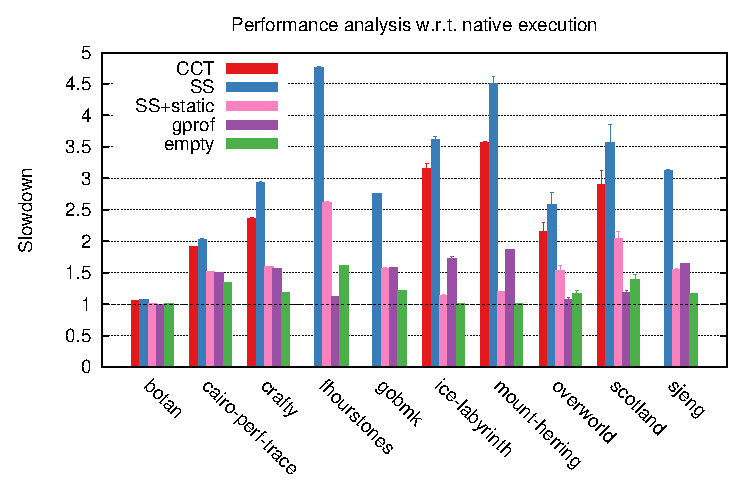
\includegraphics[width=0.49\textwidth]{figures/hcct-slowdown/hcct-slowdown-native.eps} &
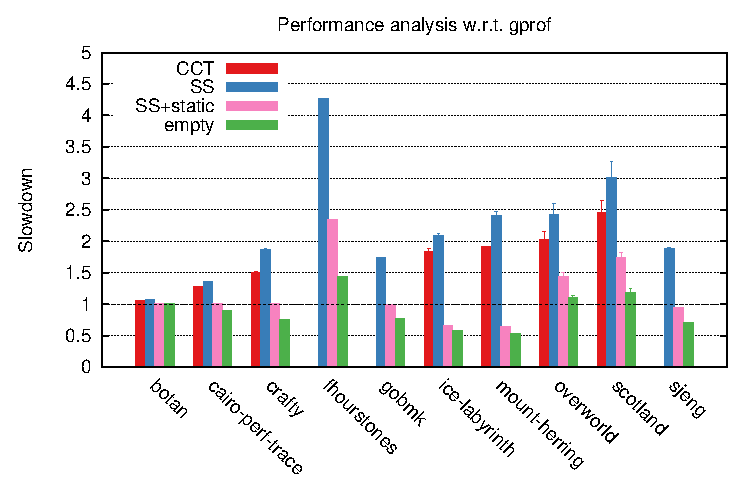
\includegraphics[width=0.49\textwidth]{figures/hcct-slowdown/hcct-slowdown-gprof.eps}\\
(a) & (b)
\end{tabular}
\caption{\protect\label{fig:hcct-slowdown} Runtime analysis for CCT and $(\phi,\varepsilon)$-HCCT construction compared to (a) native executions and (b) executions under \gprof. The {\em empty} bars measure the cost of instrumenting function calls and returns. SS with stating bursting has been executed with sampling interval 20 msec and burst length 2 msec.
}
\end{center}
\end{figure}
\fi

\noindent \myfigure\ref{fig:hcct-slowdown}(a) shows the overheads of the different profilers normalized against the performance of a native execution. The average slowdown for the CCT construction is $2.45\times$, with a peak of $3.56\times$ for {\tt mount-herring}. Note that data for benchmarks {\tt fhourstones}, {\tt gobmk} and {\tt sjeng} are not reported for the CCT profiler as it ran out of memory. We observe that the construction of the $(\phi,\varepsilon)$-HCCT incurs an average slowdown of $2.9\times$ ($3.09\times$ considering also OOM benchmarks) and is $16.28\%$ slower than the CCT profiler, with a peak of $26.08\%$ for {\tt mount-herring}. Given the previously discussed memory usage reduction and the $(\phi,\varepsilon)$-HCCT accuracy results that we will discuss in the next section, we believe this represents an interesting trade-off between time, space and precision.

The integration with static bursting reduces the average overhead of our approach to $1.58\times$ for the whole set of benchmarks, which is not far from the $1.21\times$ slowdown introduced by the {\tt gcc} instrumentation itself. We observe a peak of $2.62\times$ on the benchmark {\tt fhourstones}: we believe this is due to the particular structure of its source code, which contains very frequently invoked tiny functions that are not inlined in the experiment. %could be replaced with macros.

In \myfigure\ref{fig:hcct-slowdown}(b) we have normalized the run-time overheads against an execution under \gprof. The combination of our approach with static bursting is very effective, as it is on average $18\%$ ($5.16\%$ if we exclude {\tt fhourstones}) slower than \gprof. On 5 out of 10 benchmarks, the two tools achieve nearly-identical slowdowns. We observe $2.34\times$, $1.44\times$ and $1.74\times$ slowdowns on {\tt fhourstones}, {\tt overworld}, and {\tt scotland}, respectively. Notice that for all these benchmarks the cost of the instrumentation inserted by \gcc\ is already greater than the slowdown introduced by \gprof. On the other hand, we observe appreciable speedups on {\tt ice-labyrinth} and {\tt mount-herring}, for which SS combined with static bursting is $1.51\times$ and $1.55\times$ faster than \gprof, respectively.

\subsection{Accuracy}
\label{ss:hcct-accuracy}

\paragraph*{Exact HCCT.} We first discuss the accuracy of the exact HCCT with respect to the full CCT. Since the HCCT is a subtree of the $(\phi,\varepsilon)$-HCCT computed by our algorithms, the results described in this section apply to the $(\phi,\varepsilon)$-HCCT as well: the values of degree of overlap and hot edge coverage on the HCCT are a lower bound to the corresponding values in the  $(\phi,\varepsilon)$-HCCT, while the frequency of uncovered contexts is an upper bound.

It is not difficult to see that the cumulative distribution  of calling context frequencies shown in \myfigure\ref{fig:hcct-skewness} \ifauthorea{}{(page \pageref{fig:hcct-skewness})} corresponds exactly to the degree of overlap with the full CCT. This distribution roughly satisfies the $10\%\,$-$\,90\%$ rule: hence, with only $10\%$ of hot contexts, we have a degree of overlap around $90\%$ on all benchmarks.

\ifdefined\noauthorea
\begin{figure}[!ht]
\begin{center}
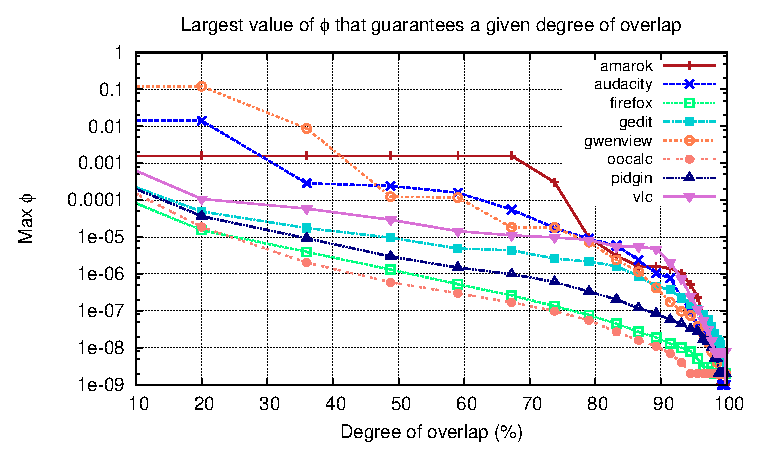
\includegraphics[width=0.65\textwidth]{figures/hcct-overlap/hcct-overlap.eps}
\caption{\protect\label{fig:hcct-overlap} Relation between $\phi$ and degree of overlap between the exact HCCT and the full CCT on a representative subset of benchmarks.
}
\end{center}
\end{figure}
\fi

\noindent \myfigure\ref{fig:hcct-overlap} illustrates the relation between degree of overlap and hotness threshold, plotting the value $\widetilde\phi$ of the largest hotness threshold for which a given degree of overlap $d$ can be achieved: using any $\phi\leq\widetilde\phi$, the achieved degree of overlap will be larger than or equal to $d$. The value of $\widetilde\phi$ decreases as $d$ increases: if we want to achieve a larger degree of overlap, we must include in the HCCT a larger number of nodes, which corresponds to choosing a smaller hotness threshold. However, when computing the $(\phi,\varepsilon)$-HCCT, the value of $\phi$ indirectly affects the space used by the algorithm and in practice cannot be too small (see \mysection\ref{ss:hcct-experimental-setup}). By analyzing hot edge coverage and uncovered frequency, we show that even when the degree of overlap is not particularly large, the HCCT and the $(\phi,\varepsilon)$-HCCT are nevertheless good approximations of the full CCT.

As shown in \myfigure\ref{fig:hcct-space-by-phi,fig:hcct-coverage}, for values of $\phi$ as small as $10^{-4}$ the space usage is less than $1\%$ of the full CCT, while guaranteeing 100\% coverage for all edges with hotness at least 10\% on most benchmarks. Smaller values of $\phi$ increase space and improve the degree of overlap, but are unlikely to be interesting in applications that require mining hot calling contexts.

Notice that $\phi=10^{-4}$ yields a degree of overlap as small as $10\%$ on two of the less skewed benchmarks ({\tt oocalc} and {\tt firefox}), which seems to be a bad scenario. However, \myfigure\ref{fig:hcct-uncovered} analyzes how the remaining $90\%$ of the total CCT weight is distributed among uncovered contexts: the average frequency of uncovered contexts is about $0.01\%$ of the frequency of the hottest context, and the maximum frequency is typically less than $10\%$. This suggests that uncovered contexts are likely to be uninteresting with respect to the hottest contexts, and that the distribution of calling context frequencies obeys a ``long-tail, heavy-tail'' phenomenon: the CCT contains a huge number of calling contexts that rarely get executed, but overall these low-frequency contexts account for a significant fraction of the total CCT weight.

\ifdefined\noauthorea
\begin{figure}[!ht]
\begin{center}
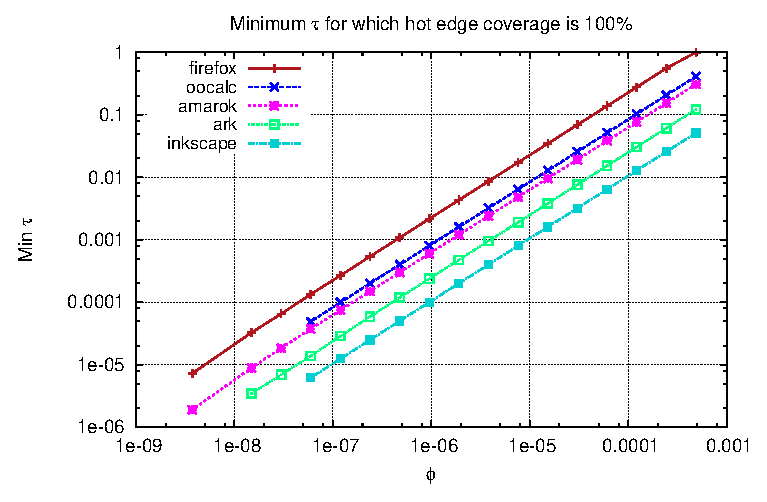
\includegraphics[width=0.65\textwidth]{figures/hcct-coverage/hcct-coverage.eps}\\
\caption{\protect\label{fig:hcct-coverage} Hot edge coverage of the exact HCCT: relation between $\phi$ and edge--weight threshold $\tau$ on a representative subset of benchmarks.
}
\end{center}
\end{figure}
\fi

\ifdefined\noauthorea
\begin{figure}[!ht]
\begin{center}
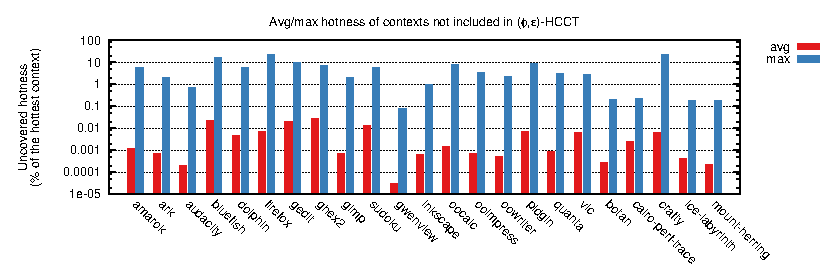
\includegraphics[width=0.95\textwidth]{figures/hcct-uncovered/hcct-uncovered.eps}\\
\caption{\protect\label{fig:hcct-uncovered} Maximum and average hotness of calling contexts not included in the $(\phi,\varepsilon)$-HCCT.
}
\end{center}
\end{figure}
\fi

\noindent \myfigure\ref{fig:hcct-coverage} confirms this intuition, showing that the HCCT represents the hot portions of the full CCT remarkably well even for values of $\phi$ for which the degree of overlap may be small. The figure plots, as a function of $\phi$, the smallest value $\widetilde\tau$ of the hotness threshold $\tau$ for which hot edge coverage of the HCCT is $100\%$. Results are shown only on some of the less skewed, and thus more difficult, benchmarks. Note that $\widetilde\tau$ is directly proportional to and roughly one order of magnitude larger than $\phi$. This is because the HCCT contains all contexts with frequency $\ge\lfloor\phi N\rfloor$, and always contains the hottest context, which has weight $w_{max}$ as in the definition of hot edge coverage in \mysection\ref{ss:hcct-experimental-setup}. Hence, the hot edge coverage is $100\%$ as long as $\lfloor\phi N\rfloor\ge\tau \cdot w_{max}$, which yields $\widetilde\tau=\lfloor\phi N\rfloor/w_{max}$. The experiment shows that $100\%$ hot edge coverage is always obtained for $\tau\ge 0.01$. As a frame of comparison, notice that the $\tau$ thresholds used in~\cite{Zhuang06} to analyze hot edge coverage are always larger than $0.05$, and for those values we always guarantee total coverage.

%%% (phi,eps)-HCCT accuracy

\ifdefined\noauthorea
\begin{figure}[!ht]
\begin{center}
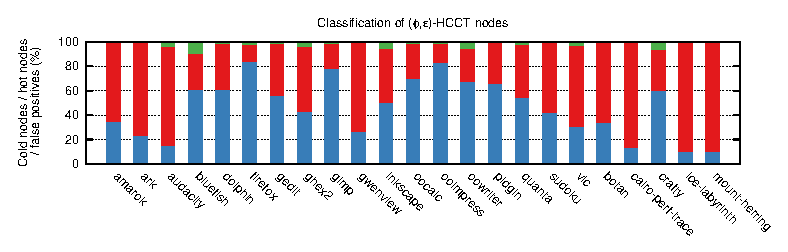
\includegraphics[width=0.95\textwidth]{figures/hcct-breakdown/hcct-breakdown.eps}\\
\caption{\protect\label{fig:hcct-breakdown} Partition of $(\phi,\varepsilon)$-HCCT nodes into: cold (bottom bar), hot (middle bar), and false positives (top bar).}
\end{center}
\end{figure}
\fi

\paragraph*{$\boldsymbol{(}\boldsymbol{\phi}\boldsymbol{,}\boldsymbol{\varepsilon}\boldsymbol{)}$-HCCT.} We now discuss the accuracy of the $(\phi,\varepsilon)$-HCCT compared to the exact HCCT. \myfigure\ref{fig:hcct-breakdown} shows the percentages of cold nodes, true hots, and false positives in the $(\phi,\varepsilon)$-HCCT using $\phi=10^{-4}$ and $\varepsilon=\phi/5$. We observe that SS includes in the tree only very few false positives: less than $10\%$ of the total number of tree nodes in the worst case, and between $0\%$ and $5\%$ for the large majority of the benchmarks. The percentage of cold nodes strictly depends on the characteristics of the particular benchmark, and is not remarkably influenced by the number of false positives, which is small.

An interesting feature of our approach is that counter estimates are very close to the true frequencies, as shown in \myfigure\ref{fig:hcct-counters}. A comparison between average and maximum errors suggests that just a few nodes are appreciably overestimated. The average counter error computed for hot contexts is actually greater than $4\%$ only for {\tt crafty}, and smaller than $2\%$ for the majority of the benchmarks.

\ifdefined\noauthorea
\begin{figure}[!ht]
\begin{center}
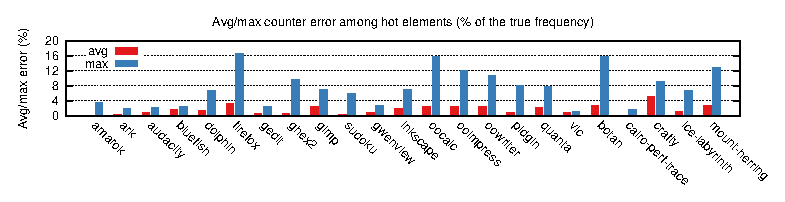
\includegraphics[width=0.95\textwidth]{figures/hcct-counters/hcct-counters.eps}\\
\caption{\protect\label{fig:hcct-counters} Accuracy of calling-context frequencies measured on hot contexts included in the $(\phi,\varepsilon)$-HCCT.}
\end{center}
\end{figure}
\fi

\noindent It is worth noticing that, when integrating SS with sampling-based approaches, the theoretical guarantees of the algorithm apply only to the stream of sampled events, and not to the full stream of routine calls and returns from the execution. For this reason, we analyze the impact of static bursting on the quality of the solution.

\noindent \myfigure\ref{fig:hcct-bursting}(a) shows the average counter error among hot calling contexts. In order to compare them with the exact frequencies from the corresponding CCTs, we adjusted the counters by dividing them by the fraction of sampled events in the stream of function calls and returns. Note that, if the stream is uniformly distributed in time, this fraction is equal to the ratio between burst length and sampling interval. While processing roughly only one tenth of the whole stream, we observe that the average counter error ranges from $6.89\%$ to $17.31\%$. An analysis of the results from the integration of static bursting with the canonical CCT construction shows very similar numbers, thus suggesting that SS does not degrade the quality of the solution.

The adoption of sampling-based techniques may cause the algorithm to miss some of the contexts with frequency very close to $\lfloor\phi N\rfloor$,  leading to some false negatives. However, our analysis of hot edge coverage reported in \myfigure\ref{fig:hcct-bursting}(b) shows that static bursting does not appreciably degrade the quality of the solution. Given the smallest $\widetilde\tau$ value for which SS guarantees $100\%$ coverage, in all of our experiments we achieve $100\%$ coverage for any $\tau\ge2\widetilde\tau$ (i.e., when $\widetilde\tau/\tau\le0.5$), and only in one case ({\tt mount-herring} benchmark) hot edge coverage drops below $90\%$.

\ifdefined\noauthorea
\begin{figure}[!ht]
\begin{center}
\begin{tabular}{cc}
\hspace{-6mm}
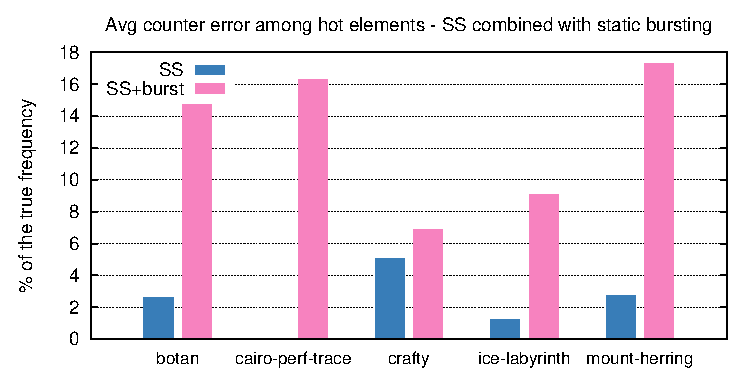
\includegraphics[width=0.49\textwidth]{figures/hcct-bursting/hcct-bursting-accuracy.eps} &
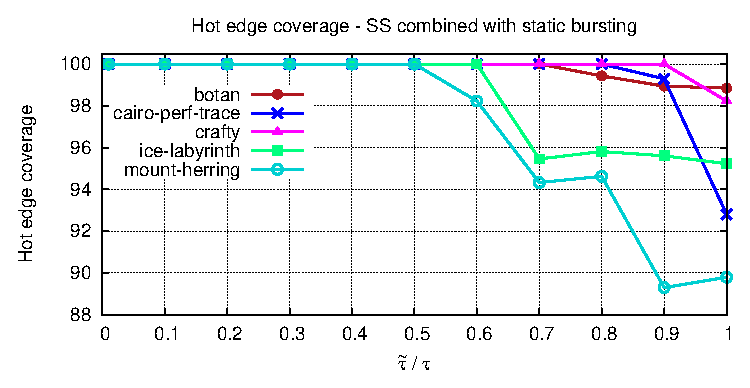
\includegraphics[width=0.49\textwidth]{figures/hcct-bursting/hcct-bursting-coverage.eps}\\
(a) & (b)
\end{tabular}
\caption{\protect\label{fig:hcct-bursting} (a) Accuracy of frequencies measured on hot calling contexts when SS is combined with static bursting. (b) Hot edge coverage for decreasing values of the hotness threshold $\tau$. As pointed out in \mysection\ref{ss:hcct-accuracy}, $\widetilde\tau$ is the minimum threshold for which SS guarantees 100\% coverage when static bursting is disabled. We chose a representative subset of benchmarks for both charts; sampling interval has been set to 20 msec and burst length to 2 msec.}
\end{center}
\end{figure}
\fi

\subsection{Discussion}
We have seen that maintaining the $(\phi,\varepsilon)$-HCCT typically requires orders of magnitude less memory compared to the CCT. Although the fraction of cold ancestors varies from one application to another, the space required by the MCCT is typically proportional to the number of monitored contexts, which for a given $\phi$ is constant in Space Saving: for this reason, the $(\phi,\varepsilon)$-HCCT scales very well to larger applications. Theoretical predictions on accuracy are reinforced by experimental results: frequency estimates are very close to the exact counts, and Space Saving achieves good precision as well (i.e., the fraction of false positives is small). An integration with static bursting to reduce the instrumentation overhead seemed like a natural choice: our results suggest that only contexts whose frequency is very close to $\phi N$ may be missed, and the error in frequency estimates due to sampling is reasonable.